%! TEX root = **/000-main.tex
% vim: spell spelllang=en:
\chapter{Analysis}
\label{sec:analysis}

% Same from Frenay
\begin{figure}
    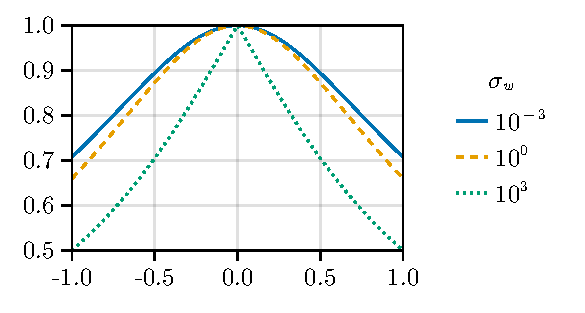
\includegraphics{plots/kernel_asin.pdf}
    \caption{Normalized Asymptotic ELM kernel evaluated around 0}
\end{figure}

% 3d version
\begin{figure}
    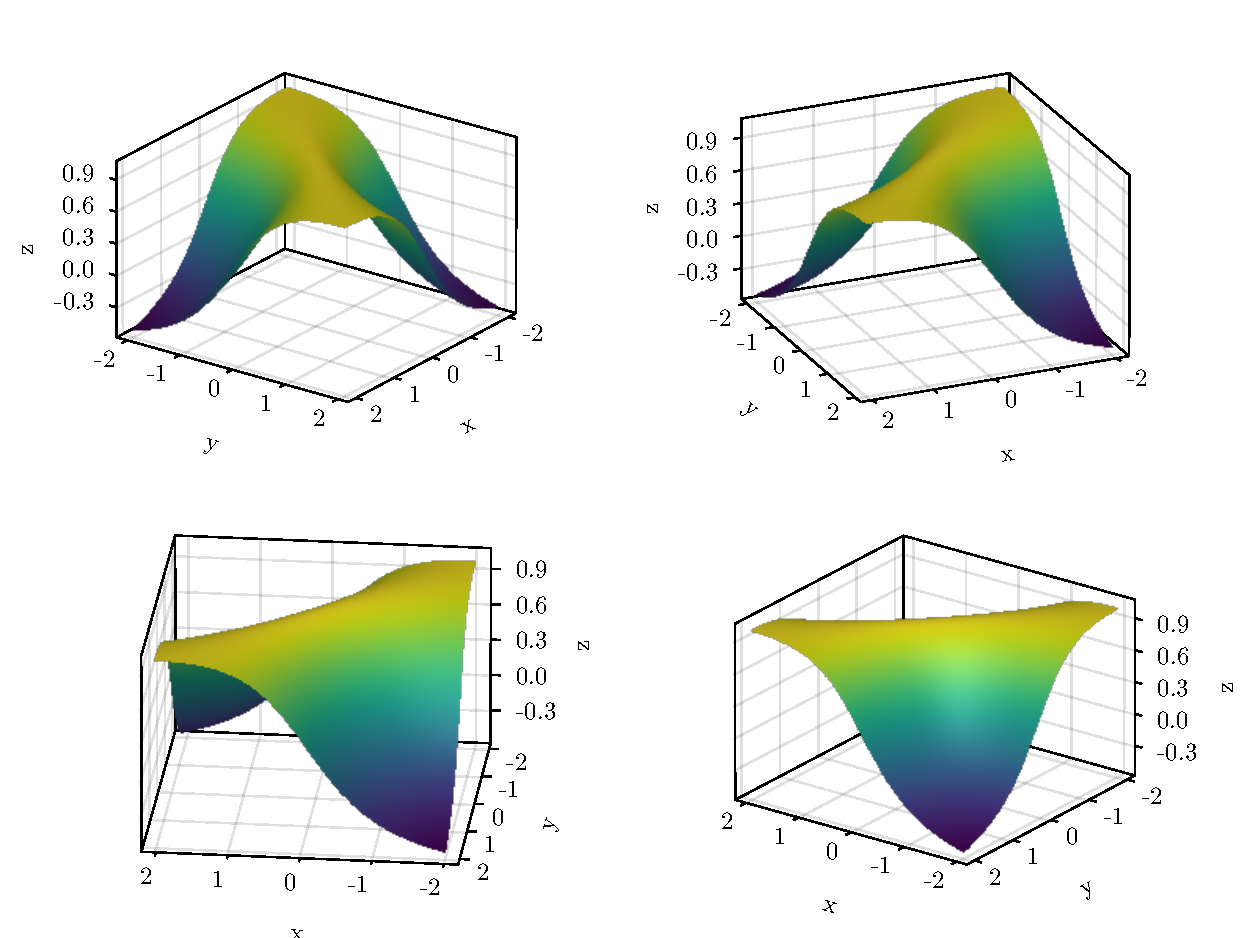
\includegraphics{plots/kernel_asin_3d_sig1}
    \caption{asin kernel with $\sigma_w=1$}
\end{figure}

\begin{figure}
    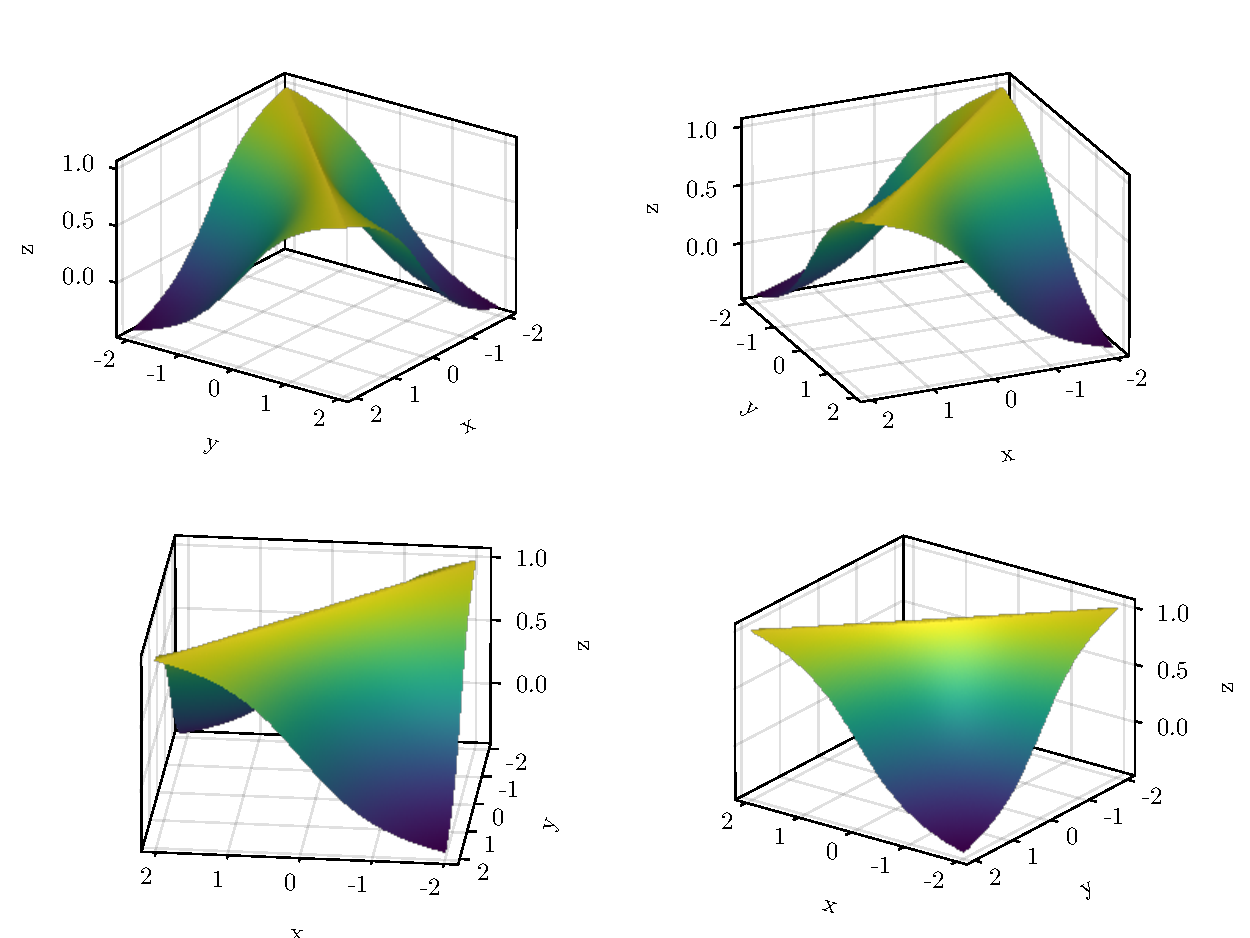
\includegraphics{plots/kernel_asin_3d_sig1000}
    \caption{asin kernel with $\sigma_w=1\,000$}
\end{figure}


% The acos ones are not very interesting with one dimensional vectors
\begin{figure}
    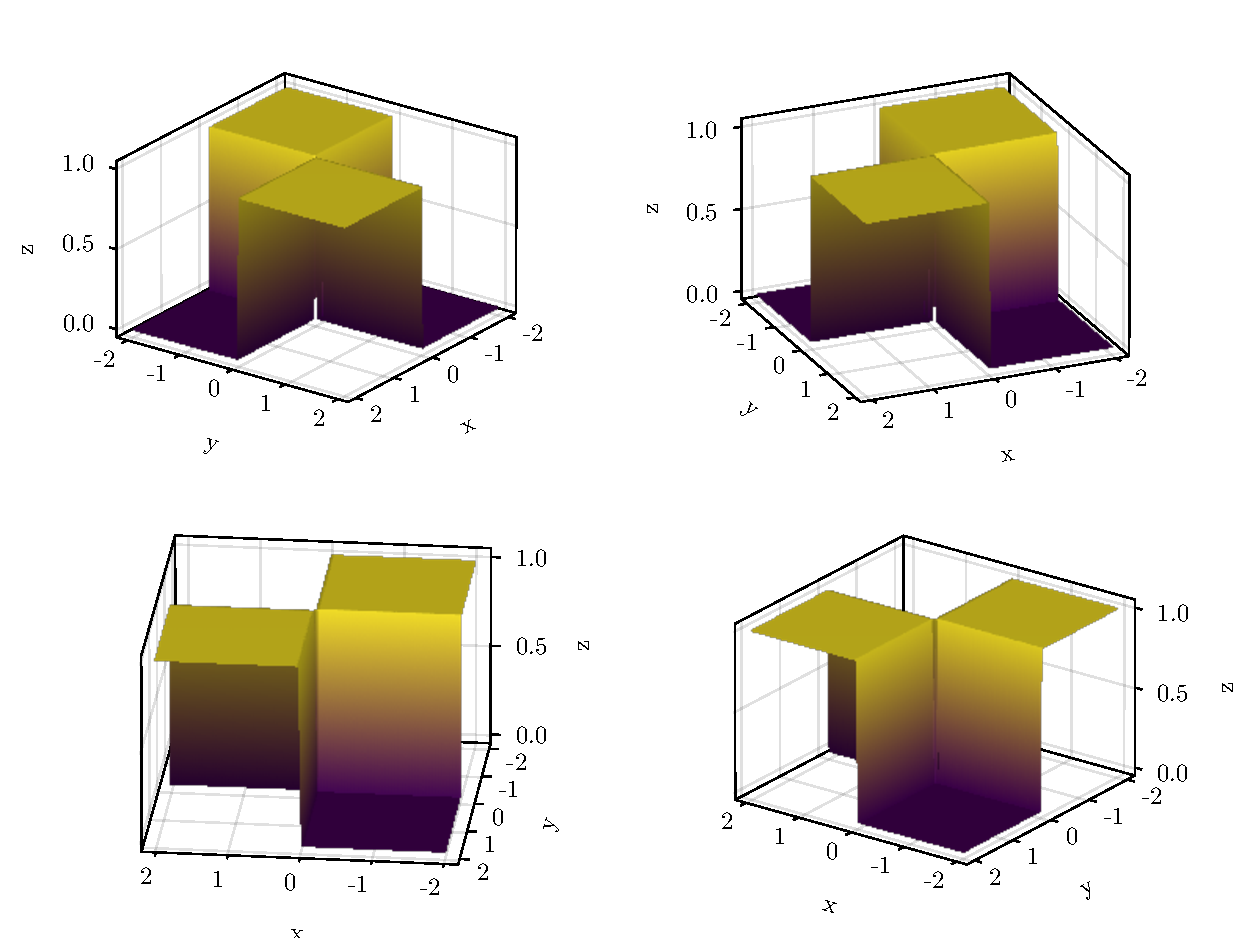
\includegraphics{plots/kernel_acos0_3d.pdf}
    \caption{acos kernel $n=0$}
\end{figure}

\begin{figure}
    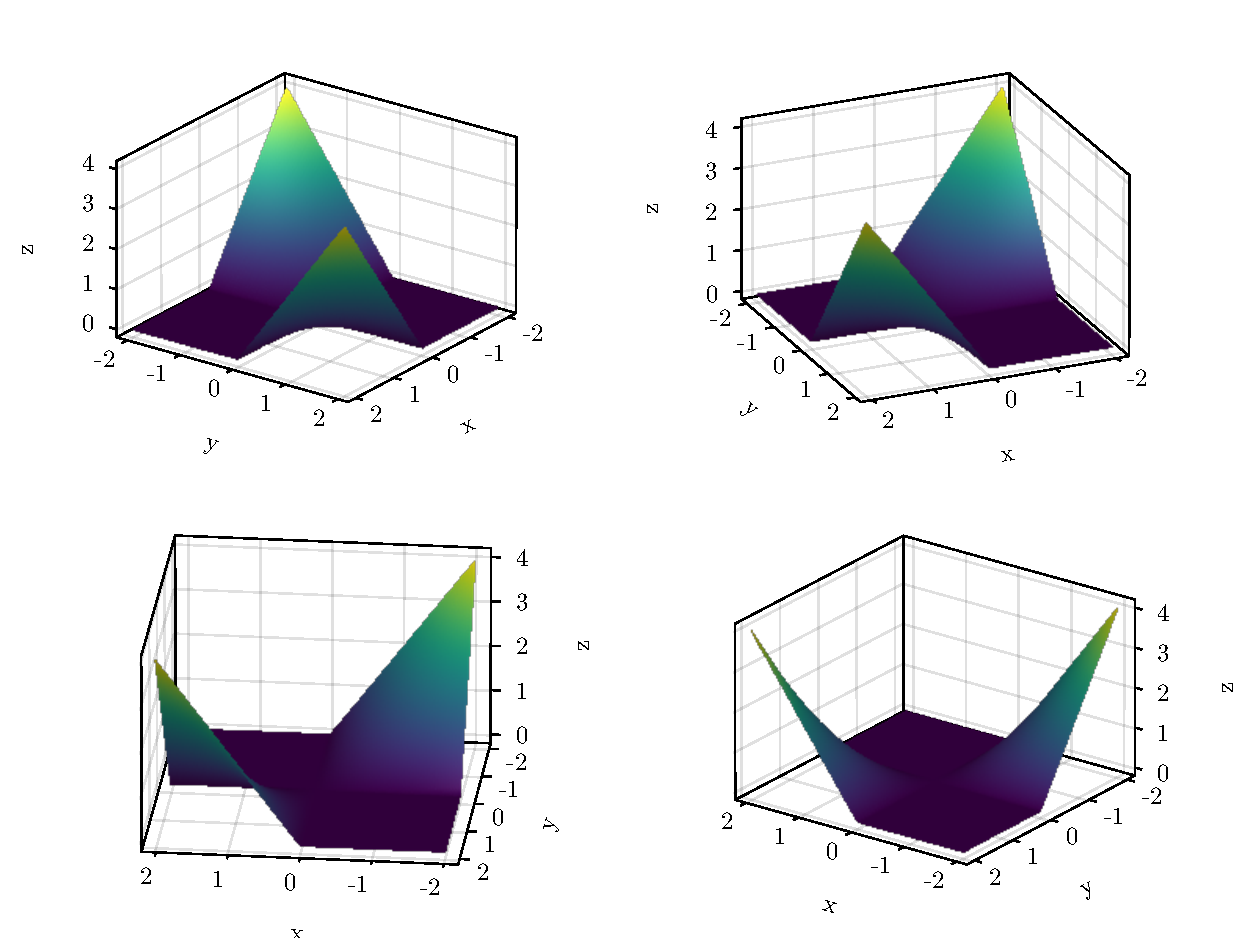
\includegraphics{plots/kernel_acos1_3d.pdf}
    \caption{acos kernel $n=1$}
\end{figure}

\begin{figure}
    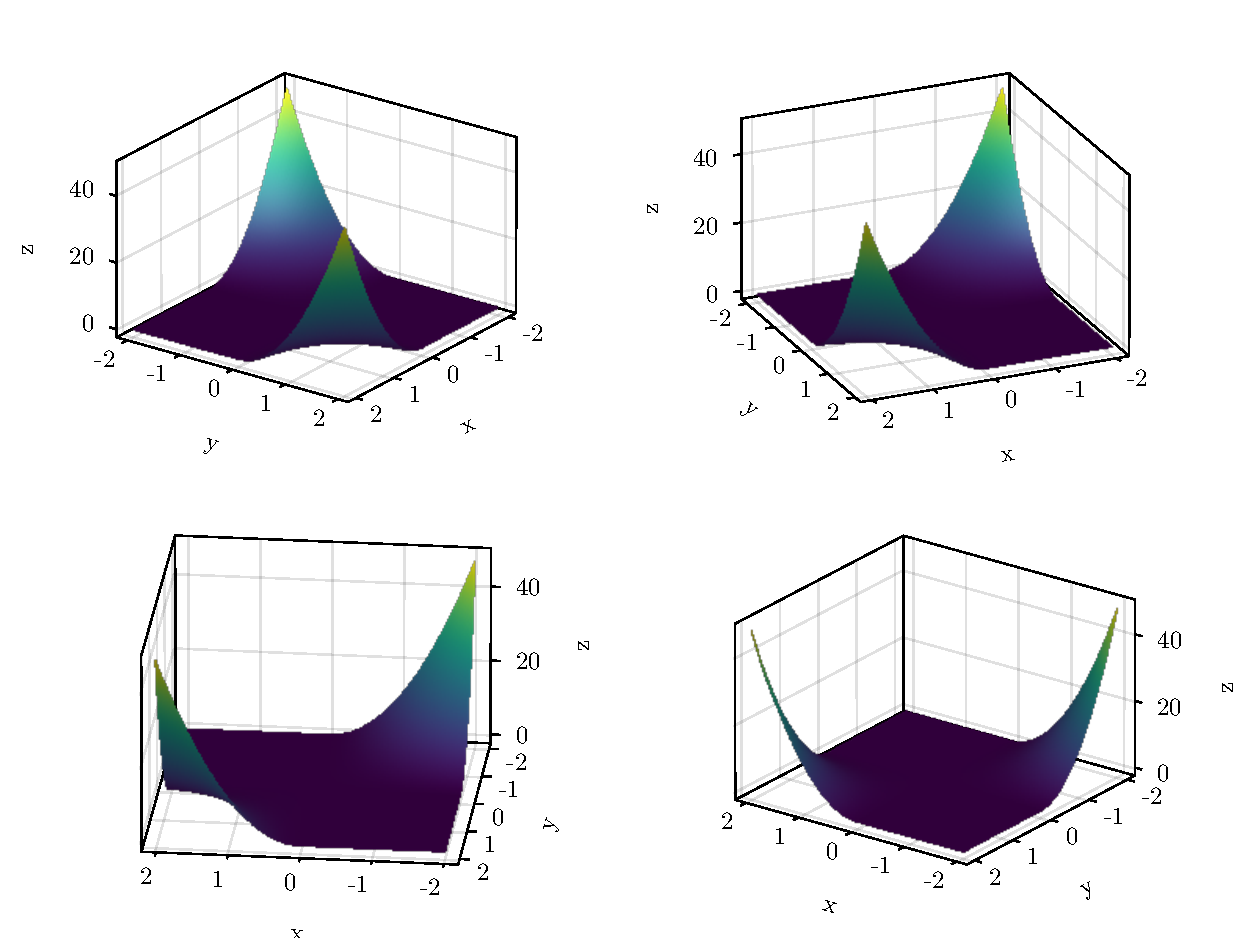
\includegraphics{plots/kernel_acos2_3d.pdf}
    \caption{acos kernel $n=2$}
\end{figure}
